% Results. Written after the results gate. Every number is a macro from numbers.tex (claims.jsonl).
% Runs: select, level-mde (with the check-methods values it echoes), h1-wage, h2-emp, h3-years,
% verdict, posthoc (deviation D7, post hoc, run unreviewed with the human's agreement).
% Rule r-ph-h1-joint: the Georgia critical-value check (r-ph-gal-*, r-ph-galnu-*, r-h1-crit-georgia,
% r-ph-ga-*, r-ph-loo-*) and the wage drift check (r-ph-wage-*) are cited only together.
\section{Results}
\label{sec:results}

Table~\ref{tab:headline} gives the answer: under the pre-specified rules the primary
specification and both named secondary analyses label the employment effect ``inconclusive'',
the first stage in weekly earnings is not supported at its pre-specified critical value, and the
comparison of year two with year one is uninformative. The rest of this section shows how each
of these follows, in the order the runs were made: the selection of the primary estimator and
the checks of the inference and power on data through 2019 (both before any post-period outcome
was read), then the three hypotheses.

\begin{table}[tbp]
\centering
\caption{Pre-specified verdicts}
\label{tab:headline}
\small
\begin{tabularx}{\linewidth}{@{}>{\raggedright\arraybackslash}p{3.3cm}rr>{\raggedright\arraybackslash}X@{}}
\toprule
Hypothesis and specification & Estimate & 95\% interval & Label (pre-specified rule) \\
\midrule
H2, employment: primary \cand{DDT-POPW-E-R50} & $\HTwoAtt$ & $[\HTwoLoNinetyFive,\ \HTwoHiNinetyFive]$ & inconclusive; not separable from a California-wide shock \\
\addlinespace
H2 rule, S1 (Clemens and coauthors' detrended DD) & $\SOneAtt$ & $[\SOneLo,\ \SOneHi]$ & inconclusive (not the headline) \\
\addlinespace
H2 rule, S2 (Dube's SDID) & $\STwoAtt$ & $[\STwoLo,\ \STwoHi]$ & inconclusive (not the headline) \\
\addlinespace
H1, weekly earnings: primary & $\HOneAtt$ & $[\HOneLoNinetyFive,\ \HOneHiNinetyFive]$ & not supported at the pre-specified critical value ($t = \HOneT$ against $\HOneCrit$) \\
\addlinespace
H3, year two minus year one: primary & $\HThreeDiff$ & $[\HThreeDiffLo,\ \HThreeDiffHi]$ & uninformative (minimum detectable effect $\MdeHThreeMax$ above 0.04) \\
\bottomrule
\end{tabularx}

\medskip
\begin{minipage}{\linewidth}\footnotesize
\emph{Notes:} Pooled 2024Q2--2026Q1 effects for California's private NAICS 722513 against the base
quarter 2023Q3, in log points; H3 compares 2025Q2--2026Q1 with 2024Q2--2025Q1. Intervals use the
placebo standard error $\max(\SEs, \SEn)$ and the critical values fixed by run \cand{level-mde}
(Table~\ref{tab:inference}). Because H1 is not supported, H2 is reported as uninformative about the
wage floor. The H2 qualifier comes from the placebo outcome (Section~\ref{sec:rob-placebo}). No
secondary analysis or robustness check has a sign category different from the primary's
($\NNotRobust$ checks), so no ``not robust to'' qualifier applies.
\end{minipage}
\end{table}

\subsection{The selected primary estimator}
\label{sec:res-select}

The selection run read only the panel truncated at 2019Q4 and was run once. It selected
\cand{DDT-POPW-E-R50}: the difference in differences with a linear trend in the gap (fitted on the
non-COVID quarters from $B-8$ to $B$, 2022Q1--2023Q3 for the real base), the population-weighted mean of the donors' log employment, and all
50 other units as donors. Its placebo RMSE is $\SelRmse$ log points, with a largest absolute
pseudo-ATT of $\SelMaxabs$. The runner-up, the same estimator with the donor aggregate
(\cand{DDT-AGG-E-R50}), has $\RmseDDTAGGERFifty$; no other candidate has the same RMSE at four
decimals, so the tie-break was not used. Table~\ref{tab:rmse} lists all 24 RMSEs, and
Figure~\ref{fig:select} shows the six pseudo-ATTs behind each. The best candidate of each other
family is the demeaned synthetic control with D20 ($\SelBestSCRmse$), SDID with D20
($\SelBestSDIDRmse$) and plain DD with population weights and R50 ($\SelBestDDRmse$). Every
trend-adjusted candidate fits better than every other candidate, and log employment fits better
than log employment per capita within every family.

\begin{table}[tbp]
\centering
\caption{Placebo RMSE of the 24 candidates at the six pseudo-dates (log points)}
\label{tab:rmse}
\small
\begin{tabular}{@{}lcccc@{}}
\toprule
& \multicolumn{2}{c}{Log employment ($E$)} & \multicolumn{2}{c}{Log employment per capita ($P$)} \\
\cmidrule(lr){2-3}\cmidrule(l){4-5}
Estimator and weighting & D20 & R50 & D20 & R50 \\
\midrule
DD, aggregate (AGG) & $\RmseDDAGGEDTwenty$ & $\RmseDDAGGERFifty$ & $\RmseDDAGGPDTwenty$ & $\RmseDDAGGPRFifty$ \\
DD, population-weighted (POPW) & $\RmseDDPOPWEDTwenty$ & $\RmseDDPOPWERFifty$ & $\RmseDDPOPWPDTwenty$ & $\RmseDDPOPWPRFifty$ \\
DDT, aggregate (AGG) & $\RmseDDTAGGEDTwenty$ & $\RmseDDTAGGERFifty$ & $\RmseDDTAGGPDTwenty$ & $\RmseDDTAGGPRFifty$ \\
DDT, population-weighted (POPW) & $\RmseDDTPOPWEDTwenty$ & $\mathbf{\RmseDDTPOPWERFifty}$ & $\RmseDDTPOPWPDTwenty$ & $\RmseDDTPOPWPRFifty$ \\
Demeaned synthetic control (SC) & $\RmseSCEDTwenty$ & $\RmseSCERFifty$ & $\RmseSCPDTwenty$ & $\RmseSCPRFifty$ \\
Synthetic DID (SDID) & $\RmseSDIDEDTwenty$ & $\RmseSDIDERFifty$ & $\RmseSDIDPDTwenty$ & $\RmseSDIDPRFifty$ \\
\bottomrule
\end{tabular}

\medskip
\begin{minipage}{\linewidth}\footnotesize
\emph{Notes:} Run \cand{select}, data through 2019Q4. RMSE$_c$ is the root mean square of
California's pooled pseudo-ATTs at the pseudo-dates 2016Q1--2017Q2, each read on the
log-employment scale. Bold: the selected candidate. D20: Dube's 20 federal-minimum states; R50:
all 50 other units. For the SC candidates, whose weights are not unique, the largest gap between
the solver's pseudo-ATTs and an independent exact solver's is at most $\ScGapSCERFifty$ log
points (report-only).
\end{minipage}
\end{table}

\begin{figure}[tbp]
\centering
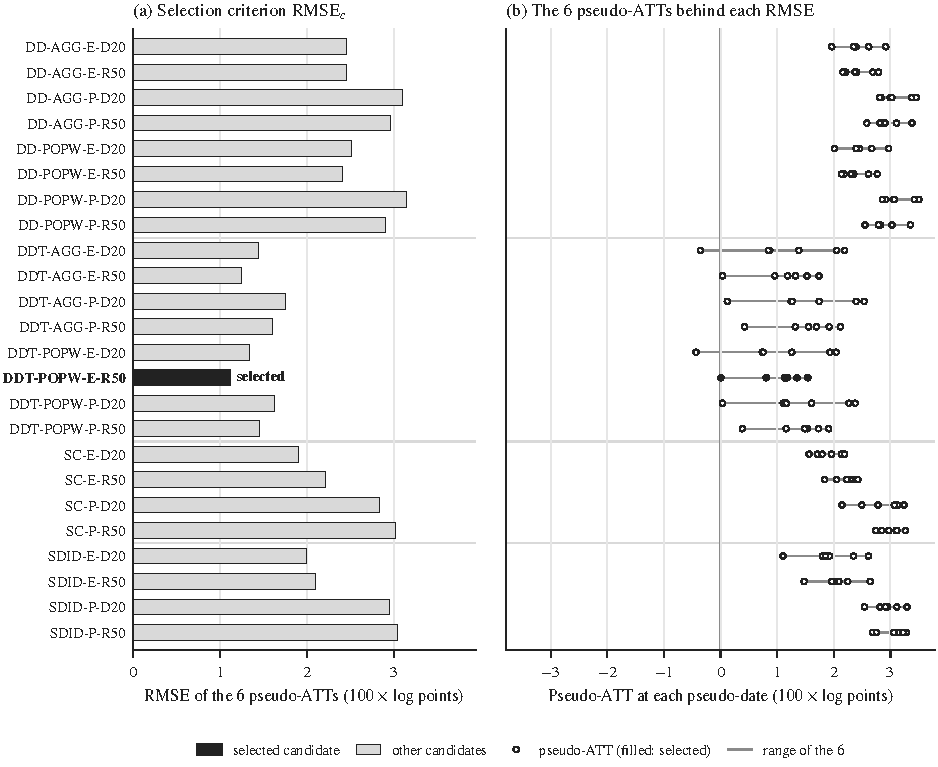
\includegraphics[width=0.88\linewidth]{figures/fig_select.pdf}
\caption{Pre-period selection of the primary estimator. Each row is one of the 24 candidates. At
each of the six pseudo-dates (2016Q1--2017Q2) California is treated as if the law had started then,
and the candidate's pseudo-ATT is its pooled estimate over the eight quarters three to ten quarters
after the pseudo-date; AB 1228 did not exist then, so a pseudo-ATT measures how far the candidate's
counterfactual misses California's path, including anything else specific to California in those
quarters, such as the rises in its general minimum wage. Panel (a): RMSE$_c$ in $100\times$ log
points (bars from zero). Panel (b): the six pseudo-ATTs behind each RMSE and their range. The
selected candidate, \cand{DDT-POPW-E-R50}, has the black bar and filled markers. The RMSEs are a
placebo criterion, not estimates with a sampling interval; the six pseudo-dates overlap, so their
pseudo-ATTs are not independent draws, and a small difference between two RMSEs is not evidence
that one estimator is better. The figure says nothing about any quarter after 2019Q4. Run
\cand{fig-select}.}
\label{fig:select}
\end{figure}

Three facts qualify the selection. First, as the design anticipated (Section~\ref{sec:select}),
the winner is a trend-adjusted candidate with the R50 pool, the kind of candidate that can track
California's own 2014--2022 general minimum-wage ramp; the rule cannot tell whether it also tracks
California's path without AB 1228 after 2023. Second, all six of the winner's employment
pseudo-ATTs are positive, from $\CaHTwoSeventeenQTwoTau$ to $\CaHTwoSixteenQTwoTau$, so most of its
RMSE is a systematic shortfall of the counterfactual, not noise. Third, the rule was applied to
employment, and H1 inherits the same estimator for wages: on log weekly wages its six pseudo-ATTs
for California are all negative, from $\CaHOneSixteenQFourTau$ to $\CaHOneSeventeenQOneTau$, so the
selected estimator fits California's pre-period wages poorly. The selected RMSE, $\SelRmse$, is
below the 2 percent bound of H2, so falsification check (i) of the identifying assumption
(Section~\ref{sec:assumption}) does not fire.

\subsection{Inference: degrees of freedom, critical values and level}
\label{sec:res-inference}

Table~\ref{tab:inference} reports, for every statistic that carries a label, the degrees of
freedom and critical values fixed by run \cand{level-mde} on data through 2019Q4, before any
post-period run. For the employment statistics of the primary (H2, H3) and of S1, the critical
values are $t$ at $\nu$: the quantiles of the decision set $L$ are less extreme. For the other-pool
check the upper ones are $t$ at $\nu$, but the lower ones, $\CritOtherPoolLoFive$ (0.05) and
$\CritOtherPoolLoTwoFive$ (0.025), come from $L$ and are more extreme than $-t_\nu$
($-\TnuOtherPoolNinetyFive$ and $-\TnuOtherPoolNinetySevenFive$), so its interval is wider on the
negative side. For H1 the quantiles of $L$ set the upper side: the upper quantiles of the 60 wage $t$ statistics in $L$,
$\LqHOneNinetyFive$ and $\LqHOneNinetySevenFive$, are far above $t_\nu$ ($\TnuHOneNinetyFive$ and
$\TnuHOneNinetySevenFive$), so they set H1's one-sided critical value and the upper end of its
interval. For S2 the SDID floor raises the upper critical values from
$\CritSTwoHiNinetyFiveNoFloor$ to $\CritSTwoHiNinetyFive$ (0.95) and from
$\CritSTwoHiNinetySevenFiveNoFloor$ to $\CritSTwoHiNinetySevenFive$ (0.975); the lower ones come
from $L$.

\begin{table}[tbp]
\centering
\caption{Degrees of freedom, critical values and level check (run \cand{level-mde}, data through 2019Q4)}
\label{tab:inference}
\small
\setlength{\tabcolsep}{3.2pt}
\begin{tabular}{@{}lrrrrrrrrrr@{}}
\toprule
& & & & & & & & \multicolumn{3}{c}{Two-sided rejection rate} \\
\cmidrule(l){9-11}
Statistic & $\nu$ & $t_{\nu,0.95}$ & $c_{\mathrm{hi}}(0.95)$ & $c_{\mathrm{hi}}(0.975)$ & $c_{\mathrm{lo}}(0.025)$ & $\mathrm{SE}_{\mathrm{pre}}$ & $k$ & all & $L$ & CA \\
\midrule
H1, wage & $\NuHOne$ & $\TnuHOneNinetyFive$ & $\CritHOneHiNinetyFive$ & $\CritHOneHiNinetySevenFive$ & $\CritHOneLoTwoFive$ & $\SePreHOne$ & $\KDiagHOne$ & $\RejHOneMaxAllTwo$ & $\RejHOneMaxSetLTwo$ & $\RejHOneMaxCATwo$ \\
H2, employment & $\NuHTwo$ & $\TnuHTwoNinetyFive$ & $\CritHTwoHiNinetyFive$ & $\CritHTwoHiNinetySevenFive$ & $\CritHTwoLoTwoFive$ & $\SePreHTwo$ & $\KDiagHTwo$ & $\RejHTwoMaxAllTwo$ & $\RejHTwoMaxSetLTwo$ & $\RejHTwoMaxCATwo$ \\
H3, year 2 $-$ year 1 & $\NuHThree$ & $\TnuHThreeNinetyFive$ & $\CritHThreeHiNinetyFive$ & $\CritHThreeHiNinetySevenFive$ & $\CritHThreeLoTwoFive$ & $\SePreHThree$ & $\KDiagHThree$ & $\RejHThreeMaxAllTwo$ & $\RejHThreeMaxSetLTwo$ & $\RejHThreeMaxCATwo$ \\
S1 & $\NuSOne$ & $\TnuSOneNinetyFive$ & $\CritSOneHiNinetyFive$ & $\CritSOneHiNinetySevenFive$ & $\CritSOneLoTwoFive$ & $\SePreSOne$ & $\KDiagSOne$ & $\RejSOneMaxAllTwo$ & $\RejSOneMaxSetLTwo$ & $\RejSOneMaxCATwo$ \\
S2 & $\NuSTwo$ & $\TnuSTwoNinetyFive$ & $\CritSTwoHiNinetyFive$ & $\CritSTwoHiNinetySevenFive$ & $\CritSTwoLoTwoFive$ & $\SePreSTwo$ & $\KDiagSTwo$ & $\RejSTwoMaxAllTwo$ & $\RejSTwoMaxSetLTwo$ & $\RejSTwoMaxCATwo$ \\
Other pool (D20) & $\NuOtherPool$ & $\TnuOtherPoolNinetyFive$ & $\CritOtherPoolHiNinetyFive$ & $\CritOtherPoolHiNinetySevenFive$ & $\CritOtherPoolLoTwoFive$ & $\SePreOtherPool$ & $\KDiagOtherPool$ & $\RejOtherPoolMaxAllTwo$ & $\RejOtherPoolMaxSetLTwo$ & $\RejOtherPoolMaxCATwo$ \\
\bottomrule
\end{tabular}

\medskip
\begin{minipage}{\linewidth}\footnotesize
\emph{Notes:} $\nu = \min(J, \hat\nu)$, the Satterthwaite degrees of freedom of $\SEn$ estimated
from the donors' pre-2020 placebo variances. $c_{\mathrm{hi}}(p)$ is the larger of $t_{\nu,p}$ and
the $p$-quantile of the 60 statistics of the decision set $L$ (the ten most populous
federal-minimum states at six pseudo-dates); $c_{\mathrm{lo}}$ likewise on the lower side; for S2
both also respect the SDID floor. $\mathrm{SE}_{\mathrm{pre}}$: root mean square of California's
standard error at the six pseudo-dates (log points). $k$: root mean square of California's six
pseudo-date $t$ statistics. Rejection rates: share of the nominal two-sided 5 percent tests that
reject with $\mathrm{SE} = \max(\SEs, \SEn)$ and $t$ at each test's own donor count, over all
pool units and California, over $L$, and over California's six tests. The binomial band around
0.05 reaches $\BandHTwoAll$ (all) and $\BandHTwoSetL$ ($L$) for the R50 statistics and
$\BandSTwoAll$ (all) for the D20 statistics. California's level is argued from the conservative
standard error, not measured: $L$ contains no state as large as California.
\end{minipage}
\end{table}

No two-sided rate over all tests or over $L$ in Table~\ref{tab:inference} is above its binomial
band. Because every donor is smaller than California, $\SEs$ is below $\SEn$ in every post-period
run, and California's standard error is $\SEn$, as the design anticipated. The one-sided rates
for California show where its own pre-period behaviour departs from the nominal level, with six
tests each: H1's lower test rejects in a share $\RejHOneMaxCALo$ of California's tests, matching
the negative wage pseudo-ATTs above, and S2's upper test in a share $\RejSTwoMaxCAUp$
(Section~\ref{sec:rob-secondary}). California's employment statistics of the primary, with
$k = \KDiagHTwo$, are small relative to their standard error, which is the conservative side.

\paragraph{Which standard error, and what the choice costs.} The H2 label depends on the
pre-specified rule $\mathrm{SE} = \max(\SEs, \SEn)$, so we report the three diagnostics the
design names for it (Section~\ref{sec:inference}). Table~\ref{tab:sechoice} gives them for the H2
statistic. First, the level check by population tercile: with the scaled $\SEs$ alone the
two-sided test rejects in a share $\RejHTwoScaledTercThreeTwo$ of the tests of the largest third
of units, the group closest to California in size, against $\RejHTwoMaxTercThreeTwo$ with the
maximum; with the unscaled $\SEn$ alone it over-rejects among the smallest third
($\RejHTwoUnscaledTercOneTwo$), where the maximum takes $\SEs$. The code-check Monte Carlo likewise
showed $\SEs$ alone over-rejecting under state-level shocks. Second, the diagnostic $k$, the root
mean square of California's own six pseudo-date $t$ statistics: $\KDiagHTwoScaled$ with $\SEs$ and
$\KDiagHTwoUnscaled$ with $\SEn$. A value of one would mean that the standard error matches
California's pre-period spread, so $\SEs$ understates that spread and $\SEn$ overstates it
severalfold; the same pattern holds for H3 ($\KDiagHThreeScaled$ against $\KDiagHThreeUnscaled$),
S1 ($\KDiagSOneScaled$ against $\KDiagSOneUnscaled$) and the other-pool check
($\KDiagOtherPoolScaled$ against $\KDiagOtherPoolUnscaled$), while for H1 ($\KDiagHOneScaled$
against $\KDiagHOneUnscaled$) and S2 ($\KDiagSTwoScaled$ against $\KDiagSTwoUnscaled$) even $\SEn$ is
close to or below California's spread. Third, Ferman and Pinto's own step, the regression of the
squared placebo estimates on a constant and $1/\mathrm{pop}_j$, which we report only as a
diagnostic: at California's six pseudo-dates its implied $\mathrm{SE}_{\mathrm{FP}}$ ranges from
$\CaHTwoSeventeenQOneFpSe$ to $\CaHTwoSixteenQOneFpSe$, against California's standard errors of
$\CaHTwoSixteenQOneSe$ to $\CaHTwoSeventeenQTwoSe$; in the real H2 run $\hat A = \HTwoFpA$ is
negative and $\hat B = \HTwoFpB$, so $\mathrm{SE}_{\mathrm{FP}} = \HTwoFpSe$: the
$A + B/\mathrm{pop}$ variance model fails here, which is not a standard error but supports not
relying on the scaled one. Read together, the diagnostics bracket California's true standard error
between $\SEs$ and $\SEn$, as the argument of Section~\ref{sec:inference} says, and show that the
maximum chosen to protect the level is far from tight for California's employment statistics. What
that costs for H2 is shown in Section~\ref{sec:res-h2}.

\begin{table}[tbp]
\centering
\caption{The H2 statistic under each standard error (run \cand{level-mde}, data through 2019Q4)}
\label{tab:sechoice}
\small
\begin{tabular}{@{}lrrrrrrr@{}}
\toprule
& \multicolumn{6}{c}{Two-sided rejection rate at nominal 5\%} & \\
\cmidrule(lr){2-7}
Standard error & Tercile 1 & Tercile 2 & Tercile 3 & All & $L$ & CA & $k$ \\
\midrule
$\SEs$ (scaled) & $\RejHTwoScaledTercOneTwo$ & $\RejHTwoScaledTercTwoTwo$ & $\RejHTwoScaledTercThreeTwo$ & $\RejHTwoScaledAllTwo$ & $\RejHTwoScaledSetLTwo$ & $\RejHTwoScaledCATwo$ & $\KDiagHTwoScaled$ \\
$\SEn$ (unscaled) & $\RejHTwoUnscaledTercOneTwo$ & $\RejHTwoUnscaledTercTwoTwo$ & $\RejHTwoUnscaledTercThreeTwo$ & $\RejHTwoUnscaledAllTwo$ & $\RejHTwoUnscaledSetLTwo$ & $\RejHTwoUnscaledCATwo$ & $\KDiagHTwoUnscaled$ \\
$\max(\SEs, \SEn)$ (pre-specified) & $\RejHTwoMaxTercOneTwo$ & $\RejHTwoMaxTercTwoTwo$ & $\RejHTwoMaxTercThreeTwo$ & $\RejHTwoMaxAllTwo$ & $\RejHTwoMaxSetLTwo$ & $\RejHTwoMaxCATwo$ & $\KDiagHTwo$ \\
\bottomrule
\end{tabular}

\medskip
\begin{minipage}{\linewidth}\footnotesize
\emph{Notes:} H2 statistic of the selected candidate (pooled log employment, R50 pool) at the six
pseudo-dates 2016Q1--2017Q2. Terciles: the pool units and California sorted by population, 1
smallest to 3 largest. $L$: the decision set; CA: California's six tests. $t$ at each test's own
donor count. $k$: root mean square of California's six pseudo-date $t$ statistics with that
standard error (one means the standard error matches California's pre-period spread).
\end{minipage}
\end{table}

Two results of the code check that preceded the design gate, echoed by run \cand{level-mde},
complete the picture. On the Proposition 99 data our exact synthetic control gives
$\PropSCsclib$ (an independent exact solve: $\PropSCexact$), and a port of the reference package's
iterative solver gives $\PropSCfwSparse$ with its default sparsification and
$\PropSCfwNoSparse$ without it, next to the printed $-19.6$ of % crew:literal
\citet[Table~1]{arkhangelsky2021synthetic}. In the Monte Carlo study, SDID with D20 donors and
pure state-level shocks rejected two-sided in a share $\McSDIDEDTwentyPureARhoZeroZeroMaxTJTwo$ of
replications at $t_J$ without autocorrelation, and $\McSDIDEDTwentyPureARhoZeroZeroFloorTwo$ with
the calibrated floor; the floor values for D20 are $\QcalDTwentyHiNinetyFive$ and
$\QcalDTwentyHiNinetySevenFive$ (upper, 0.95 and 0.975) and $\QcalDTwentyLoFive$ and
$\QcalDTwentyLoTwoFive$ (lower, 0.05 and 0.025). With unequal state-shock variances the same SDID
cell rejected in a share $\McSDIDEDTwentyHeteroARhoZeroZeroMaxTnuTwo$ even at the Monte Carlo
degrees of freedom ($\McSDIDEDTwentyHeteroARhoZeroZeroFloorTwo$ with the floor), which we report
as the size of S2's two-sided test under that design. For the selected candidate the same
unequal-variance design rejected in a share $\McDDTPOPWERFiftyHeteroARhoZeroZeroMaxTJTwo$ at
$t_J$, within its bound.

\subsection{Power, before any post-period outcome}
\label{sec:res-power}

The power quantities were computed in the same run, on data through 2019Q4, and they decided the
reach of H2 and H3 before any post-period estimate existed. The minimum detectable employment
effect at 80 percent power is $\MdeHTwo$ log points, and the half-width of the H2 90 percent
interval is $h_{90} = \HNinetyHTwo$, above the bound $b = 0.02$. The label ``no effect as large as
2\%'' (and with it ``decline smaller than 2\%'') was therefore unreachable, and the test cannot
separate the two published readings, as the design had hoped it would
(Section~\ref{sec:decision}). The probability of each label is in Table~\ref{tab:labelprob}:
``inconclusive'' had probability $\ProbTauZeroUndUndet$ with no effect and $\ProbTauAltUndUndet$
with a true decline of 3.5 percent, close to the two-year median of Clemens and coauthors. With
$t_J$ in place of $t_\nu$, which no label uses, the minimum detectable effect would be
$\MdeHTwoTJ$ and $h_{90}$ would be $\HNinetyHTwoTJ$: the degrees-of-freedom penalty is small
next to the size of the standard error. Recomputed with the real post-period standard error, the
two quantities are $\MdeHTwoPost$ and $\HNinetyHTwoPost$.

\begin{table}[tbp]
\centering
\caption{Probability of each H2 label before the post-period data were read (run \cand{level-mde})}
\label{tab:labelprob}
\small
\begin{tabularx}{\linewidth}{@{}l>{\raggedright\arraybackslash}Xrr@{}}
\toprule
Sign & Size & $\tau = 0$ & $\tau = -0.035$ \\
\midrule
negative & at least $b$: ``decline of at least 2\%'' & $\ProbTauZeroNegAtleast$ & $\ProbTauAltNegAtleast$ \\
negative & smaller than $b$: ``decline smaller than 2\%'' & $\ProbTauZeroNegSmaller$ & $\ProbTauAltNegSmaller$ \\
negative & undetermined: ``decline, size not distinguishable from 2\%'' & $\ProbTauZeroNegUndet$ & $\ProbTauAltNegUndet$ \\
undetermined & smaller than $b$: ``no effect as large as 2\%'' & $\ProbTauZeroUndSmaller$ & $\ProbTauAltUndSmaller$ \\
undetermined & at least $b$: ``inconclusive'' & $\ProbTauZeroUndAtleast$ & $\ProbTauAltUndAtleast$ \\
undetermined & undetermined: ``inconclusive'' & $\ProbTauZeroUndUndet$ & $\ProbTauAltUndUndet$ \\
positive & at least $b$: ``increase of at least 2\%'' & $\ProbTauZeroPosAtleast$ & $\ProbTauAltPosAtleast$ \\
positive & smaller than $b$: ``increase smaller than 2\%'' & $\ProbTauZeroPosSmaller$ & $\ProbTauAltPosSmaller$ \\
positive & undetermined: ``increase, size not distinguishable from 2\%'' & $\ProbTauZeroPosUndet$ & $\ProbTauAltPosUndet$ \\
\bottomrule
\end{tabularx}

\medskip
\begin{minipage}{\linewidth}\footnotesize
\emph{Notes:} From $\hat\tau = \tau + \mathrm{SE}_{\mathrm{pre}}\,T$ with $T \sim t_\nu$, the H2
critical values and $\mathrm{SE}_{\mathrm{pre}}$ of Table~\ref{tab:inference}; $\tau$ in log
points.
\end{minipage}
\end{table}

For the other two hypotheses the power run was as decisive. The minimum detectable
year-two-minus-year-one difference is $\MdeHThree$ log points, above the pre-specified threshold
of 0.04, so H3 was uninformative by rule whatever its estimate. The minimum detectable wage effect
is $\MdeHOne$, large because H1's critical value comes from the upper quantile of $L$.

\subsection{H1: weekly earnings}
\label{sec:res-h1}

The pooled 2024Q2--2026Q1 effect on California's log average weekly wage in 722513 is $\HOneAtt$
log points ($\HOnePct$ percent; about \$$\HOneDollars$ a week at the 2023Q3 level of
\$$\AwwCaBase$), with standard error $\HOneSe$ and $t = \HOneT$. The pre-specified one-sided 5
percent critical value is $\HOneCrit$, the 0.95 quantile of the decision-set wage statistics, so
the test does not reject and H1 is not supported. With $t$ at $\nu = \HOneNu$ alone the critical
value would have been $\TnuHOneNinetyFive$, and the one-sided $p$-value from $t_\nu$ is
$\HOnePUpper$, which we report for information only. The 90 percent interval is $\HOneLoNinety$
to $\HOneHiNinety$ and the 95 percent interval $\HOneLoNinetyFive$ to $\HOneHiNinetyFive$. By year,
the effect is $\HOneAttYrOne$ ($t = \HOneTYrOne$) in 2024Q2--2025Q1 and $\HOneAttYrTwo$
($t = \HOneTYrTwo$) in 2025Q2--2026Q1; the yearly tests use the pooled critical values (deviation
D5), and neither rejects. Weekly earnings per job are not the hourly wage the law sets, and nominal
wages carry differential price changes.

Three consequences follow from the design's rules. The verdict is ``not supported at the
pre-specified L-calibrated critical value'', which is not a finding that weekly earnings did not
rise. Because H1 is not supported, the employment result of H2 is reported as uninformative about
the wage floor. And the own-wage elasticities, pooled and by year, are not computed, because the
design computes them only for windows whose wage test rejects.

\paragraph{Post hoc checks of the H1 verdict (deviation D7).}
\label{sec:res-posthoc}
The results review traced the H1 critical value, and the crew then ran two report-only checks,
added after every post-period result had been seen. They come from one run, \cand{posthoc}, whose
code passed the last code review round but was changed afterwards to fix that round's minor
findings; with the human PI's agreement it was run without a further review; the ledger counts it among the analysis runs not covered by a passing
code review ($\CrewRunsUnreviewed$ in all). The two
checks point in opposite directions, and we report them only together.

The first concerns the critical value. Georgia's largest decision-set wage $t$ statistic is
$\PhGaTmax$; the other nine states' 54 tests reach at most $\PhOthersTmax$, below $t_\nu$. Georgia's published 722513 average weekly wage fell from \$$\PhGaAwwLimSvcTwoZeroOneFourQFour$
in 2014Q4 to \$$\PhGaAwwLimSvcTwoZeroOneFiveQOne$ in 2015Q1, and its year-over-year log change
less the median state's was as low as $\PhGaDevMin$ in 2015, against a largest deviation of
$\PhLargestOtherDev$ in any other state and quarter of 2015--2019; the trend windows of the 2016
pseudo-dates straddle that drop. In 2015Q1 Georgia's 722513 employment changed by
$\PhGaEmpYoyDevLimSvcTwoZeroOneFiveQOne$ relative to the median state and its 722513 establishment
count by $\PhGaEstYoyLimSvcTwoZeroOneFiveQOne$ year over year, and the weekly wages of its
full-service restaurants and of all its industries by $\PhGaAwwYoyDevFullSvcTwoZeroOneFiveQOne$
and $\PhGaAwwYoyDevTotalTwoZeroOneFiveQOne$ relative to the median; no Georgia state row of these
series is suppressed in 2014--2016. These are facts about the series; the run does not judge whether the
drop is a reporting artefact. With Georgia's own six decision-set tests removed (Georgia remaining
a donor and placebo unit), the upper decision-set quantiles fall to $\PhGaLLqNinetyFive$ and
$\PhGaLLqNinetySevenFive$, H1's critical value becomes $t_\nu = \PhGaLCritHiNinetyFive$, and the
pooled, year-one and year-two wage statistics all exceed it; the pooled 95 percent interval becomes
$\PhGaLPooledLo$ to $\PhGaLPooledHi$. Recomputing $\nu$ without Georgia's placebo variance, the
largest single share of the donors' total ($\PhGaSTwoShare$), gives $\nu = \PhNuGaOut$, a critical
value of $\PhGaLNuCritHiNinetyFive$ and a pooled interval from $\PhGaLNuPooledLo$ to
$\PhGaLNuPooledHi$. Leaving out each of the ten decision-set states in turn, only Georgia's removal
moves the critical values. But Georgia was singled out after the results were seen.

The second concerns the wage counterfactual. For the selected trend-adjusted estimator the
2022Q1--2023Q3 event-path gaps are the trend's own fit points, so the design's out-of-fit evidence
before the law is the 2014--2019 segment of the path. There the wage gap rises from
$\PhDriftWageGapStart$ in 2014Q1 to $\PhDriftWageGapEnd$ in 2019Q4, an OLS slope of
$\PhDriftWageSlope$ log points per quarter, with a root mean square of $\PhDriftWageRms$. If that
relative trend, rather than the 2022--2023 one the estimator removes, applied after 2023Q3, it
would account for
$\PhDriftWageImpliedPost$ log points at the post window's mean horizon of 6.5 quarters, against the
H1 estimate of $\HOneAtt$. But a linear extrapolation is not a test, and the 2014--2019 segment
contains California's own general minimum-wage ramp, so which relative trend applies after 2023Q3
is not identified.

Read together, the first check says that the pre-specified critical value is set by one state's
series and the second that the wage estimate may partly reflect a relative trend the estimator
does not remove. Neither changes the pre-specified verdict, and neither licenses the reading that
the first stage is established or that it is absent.

\subsection{H2: employment}
\label{sec:res-h2}

The pooled 2024Q2--2026Q1 effect on California's seasonally adjusted log employment in private
722513 is $\HTwoAtt$ log points, or $\HTwoPct$ percent. At California's mean post-window employment
of $\CaEmpPost$ that is about $\HTwoJobs$ jobs, with a 95 percent interval from $\HTwoJobsLo$ to
$\HTwoJobsHi$. The placebo standard error is $\HTwoSe$, the unscaled one ($\SEs = \HTwoSeScaled$),
and with $\nu = \HTwoNu$ the 95 percent interval is $\HTwoLoNinetyFive$ to $\HTwoHiNinetyFive$
($\HTwoPctLo$ to $\HTwoPctHi$ percent) and the 90 percent interval $\HTwoLoNinety$ to
$\HTwoHiNinety$. The 95 percent interval contains zero, so the sign is undetermined; the 90 percent
interval reaches beyond $\pm0.02$, so the size is undetermined; the label is ``inconclusive''. The
two-sided $p$-value from $t_\nu$, for information, is $\HTwoPTwo$. Figure~\ref{fig:placebo} places
California's estimate among the placebo estimates of its 50 donors.

The label rests on the pre-specified choice of the larger standard error. As a report-only note,
not the pre-specified inference: with the scaled $\SEs$ alone ($\HTwoSeScaled$, the population
scaling Dube uses) in place of $\max(\SEs, \SEn)$ and the same critical values, which for H2 are
$t$ at $\nu$, the 95 percent interval of the H2 estimate would lie entirely below zero. The design
takes the larger standard error because $\SEs$ alone over-rejects for large units in the level
check ($\RejHTwoScaledTercThreeTwo$ in the largest tercile, against $\RejHTwoMaxTercThreeTwo$ with
the maximum; Table~\ref{tab:sechoice}) and under state-level shocks in the Monte Carlo study. The
``inconclusive'' label is therefore a property of this design's conservative inference for one
treated state, not of the QCEW data alone: the width of the interval is set by the standard error
the design chose to protect the level of its tests.

The verdict run qualified the label: the placebo outcome, employment outside 722513, has a 95
percent interval that excludes zero (Section~\ref{sec:rob-placebo}), so the headline is
``inconclusive; not separable from a California-wide shock''. California's employment outside
722513 ran above its counterfactual, so a deviation shared by 722513 would bias the H2 estimate
toward zero or upward, not toward a decline; no adjustment is made, since none was pre-specified.
As H1 is not supported, H2 is also uninformative about the wage floor.

The label is the one the power run made likely before the data were read, and it is not evidence
against either published estimate: Clemens and coauthors' two-year median of about $-3.5$ percent
and Dube's near-zero estimate both lie well inside the interval, although neither is the same
estimand as ours (Section~\ref{sec:lit-estimates}).

\begin{figure}[tbp]
\centering
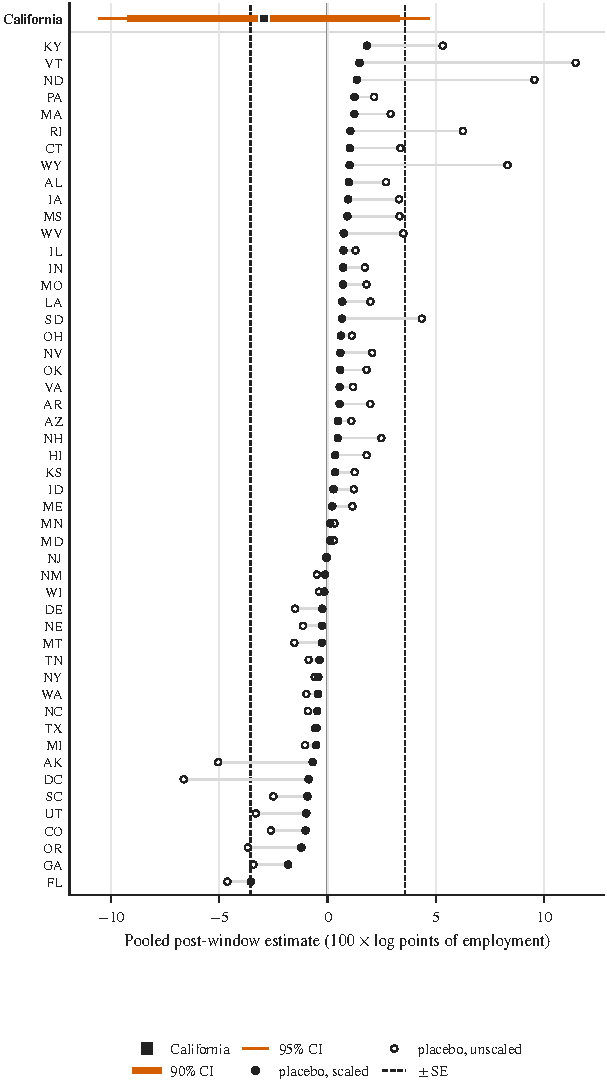
\includegraphics[width=0.52\linewidth]{figures/fig_placebo.pdf}
\caption{California's pooled H2 estimate against the placebo estimates of its 50 donors. Outcome:
seasonally adjusted log employment, NAICS 722513; estimator \cand{DDT-POPW-E-R50}; base 2023Q3, post
window 2024Q2--2026Q1; $100\times$ log points. Each donor's placebo is the same estimate with that
donor treated and the other 49 donors as its pool. Open markers: the placebo estimate; filled
markers: the same times $\sqrt{\mathrm{pop}_j/\mathrm{pop}_{\mathrm{CA}}}$. The inference uses
$\mathrm{SE} = \max(\SEs, \SEn)$, here $\SEn$; dashed lines mark $\pm\mathrm{SE}$. California's 90
percent (thick) and 95 percent (thin) intervals use the H2 critical values ($t$ at
$\nu = \HTwoNu$). The donors' placebos are not effects of any policy, the figure is not a
permutation test, and no $p$-value is read from California's rank. Run \cand{fig-placebo}.}
\label{fig:placebo}
\end{figure}

\subsection{H3: year two against year one}
\label{sec:res-h3}

The employment effect is $\HThreeYrOne$ in year one (95 percent interval $\HThreeYrOneLo$ to
$\HThreeYrOneHi$) and $\HThreeYrTwo$ in year two ($\HThreeYrTwoLo$ to $\HThreeYrTwoHi$). Their
difference is $\HThreeDiff$, with standard error $\HThreeDiffSe$ and 95 percent interval
$\HThreeDiffLo$ to $\HThreeDiffHi$. Without the power rule the H3 rule would label it ``no detectable
change''; but the minimum detectable difference is $\MdeHThree$ with the pre-period standard error
and $\MdeHThreePost$ with the real one, and the larger, $\MdeHThreeMax$, exceeds 0.04, so H3 is
``uninformative''. The yearly wage effects next to which H3 was to be read, $\HOneAttYrOne$ and
$\HOneAttYrTwo$, are not supported by their tests either, and no yearly elasticity is computed.
The data cannot say whether the effect changed as the law's premium over the general minimum fell.
